\section{Methodology}

[Development of full-core SERPENT MODELS AND OTHER THINGS ANDREI DID]

Then we perform continuous reprocessing analysis on the developed
SERPENT models using Saltproc. The reprocessing scheme is as follows:

[Reprocessing scheme - if different for reactor, mention it]

Note that some reactors have two regions, a driver and a blanket region.
Saltproc is capable of reprocessing from one region and inputting
the separated flow to the other region. For example, plutonium is bred
in the blanket region of a MCSFR, which is separated and input into
the driver region. 

Saltproc also has a reactivity control model, which controls the reactivity
by controlling the amount of fissile material put into the core. At
every depletion step, the k-eff value is checked and modifications
to the fissile stream is made accordingly.


We run the Saltproc for the entire fuel cycle of each \gls{MSR}. For example,
if a \gls{MSR} design asks for a salt-flush (complete unloading of core)
every ten years, the fuel cycle time of the \gls{MSR} would be ten years.
This way, the entire material flow history of the \gls{MSR} is captured
in the Saltproc output database.

The output database is then loaded into the Cyclus module.
The module reads the timestep of the database and the timestep of Cyclus,
and outputs the corresponding waste and surplus fissile stream every timestep.
The module also requests the corresponding amount of fertile material
that the reactor needs from the market. In short, the purpose of the module is to
mimic the interaction of a \gls{MSR} with the market, while producing
power. The module's interaction with the framework is illustrated in
figure \ref{fig:msr_int}.


\begin{figure}[htbp!]
    \begin{center}
        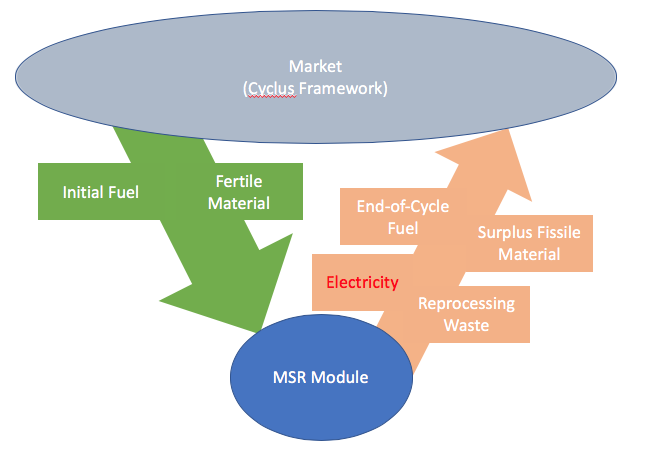
\includegraphics[scale=0.5]{./images/msr_flowchart.png}
    \end{center}
        \caption{Interaction of Cyclus \gls{MSR} module with the Cyclus framework (Market)}
    \label{fig:msr_int}
\end{figure}
